\documentclass[PredictiveAnalytics101.tex]{subfiles} 
\begin{document}
\begin{frame}
	\begin{figure}
\centering
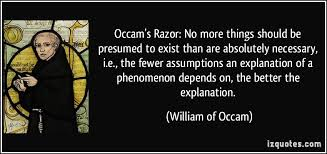
\includegraphics[width=0.99\linewidth]{occamrazor}


\end{figure}

\end{frame}

\section{Theoretical Aspects of Fitting Models}

%================================================ %
\begin{frame}
	\Large
	\frametitle{The Law of Parsimony}
	\textbf{Ockham's Razor}
	\begin{itemize}
		\item Ockham's razor, sometimes known as the law of parsimony, is simply a maxim that states that simple explanations are usually better than complicated ones. \item \textbf{Ockham's razor} was originally proposed by a monk named William of Ockham. (He did not call it "Ockham's razor" or even "my razor." This is a name that has been given to it over time.)
	\end{itemize}
	
\end{frame}
%================================================ %
\begin{frame}
	\Large
	\begin{itemize}
		\item Another version of this principle is the Law of Parsimony . This says that if you are choosing between two theories, choose the one with the fewest assumptions. 
		\item Assumptions here means claims of fact that have no evidence.
		\item A theory that doesn't have many assumptions, and is very simple, is called a parsimonious theory.
	\end{itemize}
\end{frame}
%================================================ %
\begin{frame}
	\frametitle{Law of Parsimony} 
	\Large
	\textbf{Law of Parsimony}\\
	In the context of statistics, the law of parsimony can be interpreted as an adequate model which requires the fewest independent variables is the preferred model.
\end{frame}
%================================================ %
\begin{frame}
	\Large
	\frametitle{Model building}
	\begin{itemize}
		\item The traditional approach to statistical model building is to find the most parsimonious model that still explains the data. 
		\item The more variables included in a model (overfitting), the more likely it becomes mathematically unstable, the greater the estimated standard errors become, and the more dependent the model becomes on the observed data. 
	\end{itemize}
\end{frame}
%================================================ %
\begin{frame}
	\Large
	\frametitle{Model building}
	\begin{itemize}
		\item Choosing the most adequate and minimal number of explanatory variables helps to find out the main sources of influence on the response variable, and increases the predictive ability of the model. 
		\item As a rule of thumb, there should be more than 10 observations for each variable in the model.
	\end{itemize}
	%
	%The usual procedures used in variable selection in regression analysis are: univariate analysis of each variable (using C2 test), stepwise method (backward or forward elimination of variables; using the deviance difference), and best subsets selection. Once the essential main effects are chosen, interactions should be considered next. As in all model building situations in biostatistics, biological considerations should play a role in variable selection.
	
\end{frame}
%================================================ %
\begin{frame}
	\frametitle{Overfitting}
	\Large
	\textbf{Overfitting}
	\begin{itemize}
		\item Overfitting occurs when a statistical model does not adequately describe of the underlying relationship between variables in a regression model. 
		\item When overfitting happens, the model predicts the fitted data very well, but predicts future observations poorly.
	\end{itemize}
\end{frame}
%================================================ %
\begin{frame}
	\frametitle{Overfitting}
	\Large
	\textbf{Overfitting}
	\begin{itemize}
		\item 
		Overfitting generally occurs when the model is excessively complex, such as having too many parameters (i.e. predictor variables) relative to the number of observations. 
		\item A model which has been overfit will generally have poor predictive performance, as it can exaggerate minor fluctuations in the data.
	\end{itemize}
	
	%\section{Overfitting}
	%A modeling error which occurs when a function is too closely fit to a limited set of data points. Overfitting the model generally takes the form of making an overly complex model to explain idiosyncrasies in the data under study. In reality, the data being studied often has some degree of error or random noise within it. Thus attempting to make the model conform too closely to slightly inaccurate data can infect the model with substantial errors and reduce its predictive power.
	
\end{frame}
%================================================ %
\begin{frame}
	\frametitle{Variable-Selection Procedures}
	\textbf{ Variable Selection / Feature Selection}\\
	\begin{itemize}
		\item In regression analysis, variable-selection procedures are aimed at selecting a reduced set of the independent variables - the ones providing the best fit to the model, in keeping with the Law of Parsimony.
	\end{itemize}
	
\end{frame}
%=================================%
\begin{frame}
\begin{itemize}
\item Occam's razor (or Ockham's razor) is a principle from philosophy. Suppose there exist two explanations for an occurrence. \item In this case the simpler one is usually better. 
\item Another way of saying it is that the more assumptions you have to make, the more unlikely an explanation is. 
\item Occam's razor applies especially in the philosophy of science, but also more generally.
\end{itemize}
\end{frame}
%=================================%
\end{document}
